\documentclass{beamer}
\usepackage{geometry}
\usepackage[english]{babel}
\usepackage[utf8]{inputenc}
\usepackage{amsmath}
\usepackage{amsfonts}
\usepackage{amssymb}
\usepackage{tikz}
\usepackage{graphicx}
\usepackage{venndiagram}

%\usepackage{pgfplots}
%\pgfplotsset{width=10cm,compat=1.9}
%\usepackage{pgfplotstable}

\setlength{\headheight}{26pt}%doesn't seem to fix warning

\usepackage{fancyhdr}
\pagestyle{fancy}
\fancyhf{}

%\rhead{\small{21 May 2018}}
\lhead{\small{BECA / Dr. Huson / Mathematics}}

%\vspace{1cm}

\renewcommand{\headrulewidth}{0pt}


\title{Mathematics Class Slides}
\subtitle{Bronx Early College Academy}
\author{Chris Huson}
\date{28 August 2018}

\begin{document}

\frame{\titlepage}

%\section[Outline]{}
%\frame{\tableofcontents}
 
  \section{12.1 Drui}
  \frame
  {
    \frametitle{GQ: How do we calculate area with integration?}
    \framesubtitle{CCSS: F.IF.B.6 Calculate \& interpret the rate of change of a function}

    \begin{block}{Do Now}
    \begin{enumerate}
        \item Find $\int{(4x^3-3x+1)}\mathrm{d}x$.
        \item Find $\int e^{5x}\mathrm{d}x$.
        \item Find $\displaystyle \int \frac{1}{3x+1} \mathrm{d}x$.
    \end{enumerate}
    Homework review \#1, 5, 6 p. 302
    \end{block}
    Lesson: Reimann sums and the definite integral\\*[5pt]
    Task: Example 8, page 304\\*[5pt]
    Assessment: Calculator integration \\*[5pt]
    Homework: Exercises 9H evens p. 308
  }

  \section{12.1 Drui}
  \frame
  {
    \frametitle{GQ: How do we calculate area with definite integrals?}
    \framesubtitle{CCSS: F.IF.B.6 Calculate \& interpret the rate of change of a function}

    \begin{block}{Do Now}
    \begin{enumerate}
        \item Use a calculator to find $\displaystyle \int_0^{\frac{\pi}{2}}{\cos x}\ \mathrm{d}x$
        \item Differentiate $y=\sqrt{3x^3-x}$
        \item Find $\int{(6x^2-2x-5)}\mathrm{d}x$.
        \item Differentiate $y={(3x^2-5x)^5}$
        \item Find $\int 5(x^2+1)^4(2x)\mathrm{d}x$.
        \item Find $\displaystyle \int \frac{3}{x}\ \mathrm{d}x$.
    \end{enumerate}
    \end{block}
    Lesson: Properties of definite integrals p. 307\\%*[5pt]
    Task: Review homework problems\\%*[5pt]
    Assessment: Problem \#11 p. 300 \\%*[5pt]
    Homework: Exercises 9H evens p. 308
  }

  \section{12.1 Drui}
  \frame
  {
    \frametitle{GQ: How do we calculate area with definite integrals?}
    \framesubtitle{CCSS: F.IF.B.6 Calculate \& interpret the rate of change of a function}

    \begin{block}{Do Now}
    \begin{enumerate}
        \item Use a calculator to find $\displaystyle \int_{-1}^{1}{\frac{1}{x+2}}\ \mathrm{d}x$
        \item Differentiate $y=\sqrt[3]{5x^2-2x}$
        \item Find $\int{(6x^2-2)^4(12x)} \ \mathrm{d}x$.
        \item Differentiate $y={(3x^2-5x)(\ln x)}$
        \item Find $\displaystyle \int_1^2 \frac{3}{x^2}\ \mathrm{d}x$. (check your result with a calculator)
    \end{enumerate}
    \end{block}
    Lesson: The fundamental theorem of calculus p. 309\\%*[5pt]
    Task: Practice Examples 11, 12 p. 310-1\\%*[5pt]
    Assessment: Problem 9J \#1 p. 312 \\%*[5pt]
    Homework: Exercises 9I, 9J p. 310-12
  }

  \section{12.1 Drui}
  \frame
  {
    \frametitle{GQ: How do we calculate the area between two curves?}
    \framesubtitle{CCSS: F.IF.B.6 Calculate \& interpret the rate of change of a function}

    \begin{block}{Do Now: Consider the function $f(x)=-x^2+2x+3$}
    \begin{enumerate}
        \item Factor $f$ and state its zeros.
        \item Restate $f$ in vertex form. Write down the vertex as an ordered pair.
        \item Differentiate $f$. Show that the zero of $f^\prime(x)$ is the vertex of $f$.
        \item If $f(x)$ represents the height of a diver over the domain $0 \leq x \leq 3$, interpret $f(0)$ and $f^\prime(0)$
        \item What is the size of the area bounded by $f$, $x=0$, and $y=0$?
    \end{enumerate}
    \end{block}
    Lesson: The area between two functions p. 313\\%*[5pt]
    %Task: Practice Examples 11, 12 p. 310-1\\%*[5pt]
    Assessment: Example \#13 p. 314 \\%*[5pt]
    Homework: Exercises 9K p. 316
  }

  \section{12.1 Drui}
  \frame
  {
    \frametitle{GQ: How do we calculate a volume of rotation?}
    \framesubtitle{CCSS: F.IF.B.6 Calculate \& interpret the rate of change of a function}

    \begin{block}{Do Now: Sketch the functions $f(x)=10x+x^2-3x^3$ and $g(x)=x^2-2x$}
    \begin{enumerate}
        \item What are their intersections? (i.e. $f(x)=g(x)$)
        \item What is the definite integral representing the area between the curves?
        \item Using a calculator, what is the size of the area? (this may not be a trivial question)
    \end{enumerate}
    \end{block}
    Lesson: Integrating circle areas, modeling a solid p. 318\\%*[5pt]
    %Task: Practice Examples 11, 12 p. 310-1\\%*[5pt]
    Assessment: Example \#15 p. 319 \\%*[5pt]
    Homework: Exercises 9L \& 9M p. 317, 319; probability handout
  }

  \section{12.1 Drui}
  \frame
  {
    \frametitle{GQ: How do we calculate displacement from velocity?}
    \framesubtitle{CCSS: F.IF.B.6 Calculate \& interpret the rate of change of a function \qquad \alert{12.1}}

    \begin{block}{Do Now: Do the calculations below and read the handout}
    \begin{enumerate}
        \item Lance Armstrong’s average speed in his six Tour de France victories from 1999-2004 was about 24 miles per hour. Assuming that he pedals at his average speed and takes no breaks, how long would it take him to ride 38 miles to the top of a 10,000 ft. volcano?
        \item People who are not Lance Armstrong can travel at about 12 miles per hour on a bike. At that speed, how long would it take to reach the top of the volcano?
    \end{enumerate}
    \end{block}
    Lesson: Integrating velocity over time, displacement p. 321\\%*[5pt]
    %Task: Practice Examples 11, 12 p. 310-1\\%*[5pt]
    Assessment: Example \#18 p. 323 \\%*[5pt]
    Homework: Exercises 9N \& 9O p. 320, 324
  }

  \section{12.1 Drui}
  \frame
  {
    \frametitle{GQ: How do we calculate displacement from velocity?}
    \framesubtitle{CCSS: F.IF.B.6 Calculate \& interpret the rate of change of a function \qquad \alert{12.1}}

    \begin{block}{Do Now: continued, 38 mile ride in 10 hours}
    \begin{enumerate}
        \item Using the velocity vs time graph from yesterday, integrate to show that the areas representing the distance covered by the three riders are equal ($v \times t = d$).
        \item Show that a rider accelerating according to $v(t)= \frac{76}{100}t$ also arrives at $(10,38)$.
    \end{enumerate}
    \end{block}
    Lesson: Integrating velocity over time, displacement p. 321\\%*[5pt]
    Task: Review 9F, 9M, probability\\%*[5pt]
    Assessment: Example \#18 p. 323 (take home test Thursday)\\%*[5pt]
    Homework: Exercises 9P p. 326, any remaining problem sets
  }

  \section{12.1 Drui}
  \frame
  {
    \frametitle{GQ: How does a function's graph relate to its derivatives?}
    \framesubtitle{CCSS: HSF.IF.B.4 Interpret key features of functions and their graphs \qquad \alert{12.1}}

    \begin{block}{Do Now: Differential calculus}
    \begin{enumerate}
        \item Take the 1st \& 2nd derivatives of $f(x)=x^3-6x^2+6x$.
        \item Sketch the function.\\*
        Challenge: Identify key features, graphically \& algebraically.
    \end{enumerate}
    \end{block}
    Lesson: Function graphs, extrema, the 1st \& 2nd derivative tests p. 233, 240\\%*[5pt]
    Task: 7Q p. 232 \#1-3; 7R p. 234 1, 2; 7S p. 236 1, 3 \\%*[5pt]
    Assessment: Handout graphing problem \#1 (\#2 challenge)
    \\%*[5pt]
    Homework: IB function / graphing problem set
  }

  \section{12.1 Drui}
  \frame
  {
    \frametitle{GQ: How does a function's graph relate to its derivatives?}
    \framesubtitle{CCSS: HSF.IF.B.4 Interpret key features of functions and their graphs \qquad \alert{12.1}}

    \begin{block}{Do Now: Given $f(x)=x \cos x, 0 \leq x \leq 2\pi$.}
    \begin{enumerate}
        \item Take the 1st \& 2nd derivatives of $f(x)$. \item Sketch the function. \item Over what intervals is the function increasing, decreasing?
    \end{enumerate}
    \end{block}
    Lesson: Function graphs, extrema, the 1st \& 2nd derivative tests p. 233, 240\\%*[5pt]
    Task: 7Q p. 232 \#1-3; 7R p. 234 1, 2; 7S p. 236 1, 3 \\%*[5pt]
    Assessment: Handout graphing problem \#1 (\#2 challenge)
    \\%*[5pt]
    Homework: Test corrections Paper 1
  }

  \section{12.1 Drui}
  \frame
  {
    \frametitle{GQ: How does a function's graph relate to its derivatives?}
    \framesubtitle{CCSS: HSF.IF.B.4 Interpret key features of functions and their graphs \qquad \alert{12.1}}

    \begin{block}{Do Now: Given $f\left(x\right) =-x^4 +2x^2 +x$. There are $x$-intercepts at $x=0$ and $x=p$. There is a maximum at A where $x=a$, and a point of inflection at B where $x=b$.}
    \begin{enumerate}
        \item Find the value of $p$.
        \item Write down the coordinates of A.
        \item Write down the rate of change of $f$ at A.
        \item Find the coordinates of B.
        \item Write down the rate of change of $f$ at B.
    \end{enumerate}
    \end{block}
    Lesson: The 1st \& 2nd derivative tests p. 233, 240\\%*[5pt]
    Task: 7Q p. 232 \#1-3; 7R p. 234 1, 2; 7S p. 236 1, 3 \\%*[5pt]
    Assessment: Calculator calculus functions in Do Now.
    \\%*[5pt]
    Homework: Handout IB function / graphing problem set
  }

  \section{12.1 Drui}
  \frame
  {
    \frametitle{GQ: How does a function's graph relate to its derivatives?}
    \framesubtitle{CCSS: HSF.IF.B.4 Interpret key features of functions and their graphs \qquad \alert{12.1}}

    \begin{block}{Do Now: Find the 1st derivative of the function and solve for it's zeros as potential extrema (stationary points). Use the 1st derivative test to determine whether it is a max, min, or neither.}
    \begin{enumerate}
        \item $f(x)=x^3$.
        \item $\displaystyle f(x)=\frac{x^2-4}{x^2-1}$
    \end{enumerate}
    \end{block}
    Lesson: The 1st \& 2nd derivative tests p. 233, 240\\%*[5pt]
    Task: Homework review; 7Q p. 232 \#1-3; 7R p. 234 1, 2; 7S p. 236 1, 3 \\%*[5pt]
    Assessment: Use of the 1st \& 2nd derivative tests
    \\%*[5pt]
    Homework: Study for test \alert{tomorrow}
  }

  \section{12.1 Drui}
  \frame
  {
    \frametitle{GQ: How is the binomial expansion like a probability tree?}
    \framesubtitle{CCSS: HSS.MD.A.3 Develop a probability distribution for a random variable \qquad \alert{12.1}}

    \begin{block}{Do Now: Make a tree representing three coin flips}
    \begin{enumerate}
        \item What is the probability of each outcome?
        \item If order doesn't matter, how can the results be consolidated into a probability distribution of the total number of heads?
    \end{enumerate}
    \end{block}
    Lesson:  Binomial expansion p. 186-8\\%*[5pt]
    Task: IB exam paper problems\\%*[5pt]
    Assessment: Test corrections due Thursday (snow pending)
    \\%*[5pt]
    Homework: Complete probability problem set
  }

  \section{12.1 Drui}
  \frame
  {
    \frametitle{GQ: How do we summarize the features of a population?}
    \framesubtitle{CCSS: HSS.MD.A.3 Develop a probability distribution for a random variable \qquad \alert{12.1}}

    \begin{block}{Do Now: Given $f(x)=x^2+3x$. \\*
    (work on paper you can turn in.}
    \begin{enumerate}
        \item Find $f'(x)$.
        \item What is the equation of the tangent to $f$ at $x=1$?
        \item Plot both $f$ and the tangent on your graphing calculator.
    \end{enumerate}
    \end{block}
    Lesson:  Cumulative distributions, summative stats p. 42-72\\%*[5pt]
    Task: Grouped frequency table calculations\\%*[5pt]
    Assessment: Problem \#3 2H p. 60
    \\%*[5pt]
    Homework: Problem set, univariate data statistics
  }


  \section{12.1 Drui}
  \frame
  {
    \frametitle{GQ: How do we interpret a cumulative distribution graph?}
    \framesubtitle{CCSS: HSS.MD.A.3 Develop a probability distribution for a random variable \qquad \alert{12.1}}

    \begin{block}{Do Now: Given the data in problem \#3 2H p. 60.\\*
    (work on paper you can turn in.)}
      \begin{enumerate}
        \item Write down the modal class.
        \item Write a formula for the mean test result.
        \item Compute the mean using the calculator stats function.
      \end{enumerate}
   \end{block}
    Homework review\\*
    Lesson:  Dispersion p. 73-83, Normal distributions p. 204-216\\%*[5pt]
    Task: Problem \#1 2K p. 72\\%*[5pt]
    Assessment: Problem \#7 Review exercise p. 79
    \\%*[5pt]
    Homework: Problem set, cumulative distributions
  }



  \section{12.1 Drui}
  \frame
  {
    \frametitle{GQ: How do we use the normal curve?}
    \framesubtitle{CCSS: HSS.MD.A.3 Develop a probability distribution for a random variable \qquad \alert{12.1}}

    \begin{block}{Do Now}
      \begin{enumerate}
      \item Confirm the regression equation fit to \#4 p. 348.
      \item How would you interpret the correlation of two variables having $r=-0.65$? (p. 359)
      \item Sketch a normal curve with $X\sim N(500, 100^2)$.
      \href{https://blog.prepscholar.com/sat-standard-deviation}{link}
      \end{enumerate}
   \end{block}
    Homework review\\*
    Lesson:  Regression, residuals, least-squares, extrapolation, mean point $(\bar{x},\bar{y})$ (p. 334-359)\\*
    Normal distribution, Z-score, inverse normal (p. 538-553) \\%*[5pt]
    Task: The standard normal and Z-score problems, 15H p. 541\\%*[5pt]
    Assessment: Exercise 15H \#1 \& 5 p. 541\\%*[5pt]
    Homework: Problem set regressions, probability distributions
  }

  \section{12.1 Drui}
  \frame
  {
    \frametitle{GQ: How do we use the inverse normal function?}
    \framesubtitle{CCSS: HSS.MD.A.3 Develop a probability distribution for a random variable \qquad \alert{12.1}}

    \begin{block}{Do Now: What formulas applying to pretest problems 4c \& 4d?}
      \begin{enumerate}
      \item Given $A$ and $B$ are independent and $\mathrm{P}(A)=0.2$, $\mathrm{P}(B)=0.8$. Find $\mathrm{P}(A \cap B)$
      \item \href{https://blog.prepscholar.com/sat-standard-deviation}{SAT link}
      \end{enumerate}
   \end{block}
    Pretest packet homework review\\*
    Lesson: Chapter 15 summary p. 553\\%*[5pt]
    Task: Review exercises p. 551\\%*[5pt]
    Assessment: Exam this week\\%*[5pt]
    Homework: IB problem set
  }


  \section{12.1 Drui}
  \frame
  {
    \frametitle{GQ: How do we integrate a function?}
    \framesubtitle{CCSS: HSF.IF.B.6 Calculate and interpret the area under a function \qquad \alert{12.1}}

    \begin{block}{Do Now: Chain rule - Take the derivative of each function}
      \begin{enumerate}
      \item $f(x)=\sin{x^3}$
      \item $g(x)=\sqrt{x^4+2}$
      \item $h(x)=\ln{(x^2+1)}$
      \end{enumerate}
   \end{block}
    Lesson: Take home exam papers assessment \& review\\%*[5pt]
    Task: Work problems on board\\%*[5pt]
    Assessment: Test corrections due\\%*[5pt]
    Homework: Integration exam problems
  }

  \section{12.1 Drui}
  \frame
  {
    \frametitle{GQ: How do we calculate volume (of a rotated function)?}
    \framesubtitle{CCSS: HSF.IF.B.6 Calculate and interpret the area under a function \qquad \alert{12.1}}

    \begin{block}{Do Now: Identifying problem types. On your homework, underline the ``M1" points you earned. Examples:}
      \begin{enumerate}
      \item $X \sim B(10, 0.5)$
      \item bell curve sketch
      \item $u= \& \quad u'=$
      \end{enumerate}
   \end{block}
    Lesson: $\displaystyle \int_a^b \pi r^2 \text{d}x$\\%*[5pt]
    Task: Work homework problems on board\\%*[5pt]
    Assessment: self-reflection on mixed versus block problem sets\\%*[5pt]
    Homework: Solids of rotation \& mixed exam problems
  }


  \section{12.1 Drui}
  \frame
  {
    \frametitle{GQ: How do we use periodic functions?}
    \framesubtitle{CCSS: HSF.TF.A.3 Extend trig functions with the unit circle \qquad \alert{12.1}}

    \begin{block}{Do Now: Create a unit circle and label the standard angles with their coordinate pairs.}
      %\begin{enumerate}
      %\item $\displaystyle \int_a^b \pi f^2 %\text{d}x$
      %\item ``$u$" substitution: $u= \& \quad u'=$
      %\end{enumerate}
   \end{block}
    Homework review, particularly: \\ $\displaystyle \int_a^b \pi f^2 \text{d}x$ \&
  ``$u$" substitution: $u= \& \quad u'=$\\[5pt]
    Lesson: Periodic functions\\%*[5pt]
    Task: Work homework problems on board\\%*[5pt]
    Assessment: problem set mark scheme\\%*[5pt]
    Homework: Sine curves \& mixed exam problems
  }


  \section{12.1 Drui}
  \frame
  {
    \frametitle{GQ: How do we use periodic functions?}
    \framesubtitle{CCSS: HSF.TF.A.3 Extend trig functions with the unit circle \qquad \alert{12.1}}

    \begin{block}{Do Now: Sketch the periodic function $f(x)=\sin{x}$}
      \begin{enumerate}
      \item Label the $x$-axis with multiples of $\pi$, including standard fractions in the first quadrant
      \item Mark the $y$-axis with the values of the standard angles (positive and negative).
      \item Mark points on the curve at the standard angles.
      \end{enumerate}
   \end{block}
    Homework review\\[5pt]
    Lesson: Applications calculating the period as $\frac{2\pi}{b}$\\%*[5pt]
    Task: Work homework problems on board\\%*[5pt]
    Assessment: problem set mark scheme\\%*[5pt]
    Homework: Trig \& mixed exam problems
  }

  \section{12.1 IB Math SL Drui}
  \frame
  {
    \frametitle{GQ: How do we use periodic functions?}
    \framesubtitle{CCSS: HSF.TF.A.3 Extend trig functions with the unit circle \qquad \alert{12.1}}

    \begin{block}{Do Now: Refresh your trigonometry!}
      \begin{enumerate}
      \item Sketch the periodic functions $f(x)=\sin{x}$ and $g(x)=\cos{x}$ on the same axes
      \item Draw the unit circle, marking the standard angles and noting their trig values: $(x=\cos{\theta}, y=\sin{\theta})$.
      \item Identify the parameters of $y=a\sin{(bx-h)}+k$
      \item In your calculator graph $f(x)=\tan{x}$
      \end{enumerate}
   \end{block}
    Lesson: Homework review\\[5pt]
    Task: Work homework problems on board\\%*[5pt]
    Assessment: problem set mark scheme\\%*[5pt]
    Homework: Trig \& mixed exam problems
  }

  \section{12.1 IB Math SL Drui}
  \frame
  {
    \frametitle{GQ: How do we prepare for the IB final exams?}
    \framesubtitle{CCSS: HSF.IF.B.4 Interpret key features of functions and their graphs \qquad \alert{12.1}}

    \begin{block}{Do Now: 1st \& 2nd derivatives of a cubic function, sketch}
      \begin{enumerate}
      \item Given the function $f(x)=x^3-9x$
      \item Find $f'(x)$ and $f''(x)$.
      \item Sketch $f$ and its two derivatives on the same set of axes. Label the intersections and extrema.
      \end{enumerate}
   \end{block}
    Lesson: Last minute study practices (reflection) \\[5pt]
    Task: Homework review: Work homework problems on board\\%*[5pt]
    Assessment: Problem set and exam mark scheme\\%*[5pt]
    Homework: Prepare for final exams
  }

  \frame
  {
    \frametitle{The volume of a function rotated around the $x$-axis}
    \framesubtitle{Differentiate over $x$, but use the area of a disk defined by $A=\pi r^2$}
  \href{https://www.youtube.com/watch?v=i4L5XoUBD_Q}{video}\\
  \begin{figure}[!ht]
      \centering
      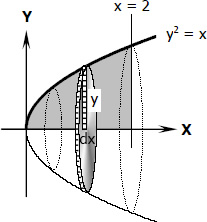
\includegraphics[width=0.5\textwidth]{0413CW-paraboloid.jpg}
  \end{figure}
  \small{Credit: MATHalino.com - Pinoy Math Community Romel Verterra}
  }

  \frame
  {
    \frametitle{Interpreting a displacement vs time graph}
    \framesubtitle{CCSS: F.IF.B.6 Calculate \& interpret the rate of change of a function}

    \begin{block}{Consider the function $f(x)=-x^2+2x+3$}
    \begin{enumerate}
        \item Factor $f$ and state its zeros.
        \item Restate $f$ in vertex form. Write down the vertex as an ordered pair.
        \item Over what intervals is the function increasing, decreasing, and neither?
        \item If $f(x)$ represents the height of a diver over the domain $0 \leq x \leq 3$, interpret $f(0)$, the vertex, and $f(3)$
        \item What does the "slope" of the curve represent?
    \end{enumerate}
    \end{block}
  }

  \section{12.1 IB Math SL Drui}
  \frame
  {
    \frametitle{GQ: How do we prepare for the IB final exams?}
    \framesubtitle{CCSS: HSF.IF.B.4 Interpret key features of functions and their graphs \qquad \alert{12.1}}

    \begin{block}{Do Now: 1st \& 2nd derivatives of a cubic function, sketch}
      \begin{enumerate}
      \item Given the function $f(x)=x^3-9x$
      \item Find $f'(x)$ and $f''(x)$.
      \item Sketch $f$ and its two derivatives on the same set of axes. Label the intersections and extrema.
      \end{enumerate}
   \end{block}
    Lesson: Last minute study practices (reflection) \\[5pt]
    Task: Homework review: Work homework problems on board\\%*[5pt]
    Assessment: Problem set and exam mark scheme\\%*[5pt]
    Homework: Prepare for final exams
  }

\end{document}
